\chapter{Stationary and signal statistics}\label{chap:stats}
\begin{overview} 
  Deterministic models of chemical engineering systems assume that all the variables are known exactly.
  However, uncertainty typically exists in the model paramters, the inputs to the model or the measurements from the model.
  This chapter summarises the nomenclature used in the rest of the work.
  The problem of estimation is also introduced briefly in addition to covering the theory used to incorporate uncertainty into models.
\end{overview}

\section{Definitions of probability}
\label{sec:statistisc:probability}
Simple random phenomena are commonly described using a model consisting of the following elements:\citep[1]{kulkarni1999modeling}
\begin{description}
\item[Sample space] Denoted $\Omega$, giving the set of all possible outcomes of the random phenomenon.  
  Particular outcomes are denoted $\omega$.
\item[Events] An event (typically denoted $E_i$) is a subset of the sample space.
\item[Event probabilities] Are written as $\prob{E}$ and are numbers between $0$ and $1$ representing the likelihood of occurrence of the event $E$.
\end{description}

Additionally, $\prob{E_2|E_1}$  represents the \emph{conditional probability} of event $E_2$ given that $E_1$ has indeed occurred.

It is clear that $\prob{\Omega}=1$, that is there is a 100\% probability of something in the set of all possible outcomes occurring.
Also, $0 \leq \prob{E_i} \leq 1 ~\forall E_i \in \Omega$ as they are probabilities.

\section{Univariate random variables}
\label{sec:univ-rand-vari}
Random variables are typically defined as the functions that map the sample space of a random phenomenon to a real number.
Examples are the value of a particular temperature or pressure or the total number of heads shown after flipping a certain number of coins.

\subsection{Cumulative distribution function}
It is often useful to refer to the cumulative distribution function (CDF) of a random variable, defined as 
\begin{equation}
  \label{eq:cdf}
  F(x) = \prob{X \leq x}, x \in (-\infty,\infty)
\end{equation}

Due to the fact that a random variable must take on a particular value in $(-\infty,\infty)$, $\lim_{x \to -\infty} F(x) = 0$ and $\lim_{x \to \infty} F(x) = 1$.
$F$ must also be nondecreasing ($x \leq y \implies F(x) \leq F(y)$) and right continuous ($\lim_{\epsilon \to 0^+} F(x+\epsilon) = F(x)$).

Random variables are called discrete if they have CDFs that contain discrete steps.  
Such discrete random variables can be characterise by their state space $S = {x_0, x_1, x_2, \dots}$.

\subsection{Probability functions}
For discrete random variables, the function $p_k = \prob{X=x_k}$ for $k \geq 0$, with $x_k \in S$ is called the probability mass function (PMF).

Random variables for which a function $f$ exist such that 
\begin{equation}
  \label{eq:cdffrompdf}
  F(x) = \int_{-\infty}^xf(u)\dd u \quad \forall x \in \mathbb{R}
\end{equation}
are called continuous random variables.
If $F$ is continuous and piecewise differentiable, then $f$ completely determines $F$ and is called the probability distribution function (PDF) of the variable $X$.
Important properties of PDFs include $f(x) \geq 0 \quad \forall x \in \mathbb{R}$ (as no negative probability integrals are allowed) and $\int_{-\infty}^{\infty} f(u) \dd u = 1$ (due to the limit on $F$).  
It is however important to note there is no upper bound on $f$.

\subsection{Expectation}
The expected value of a random variable $X$, denoted $\expect{X}$ is calculated similarly for discrete and continuous variables by summing over probability functions.  
For discrete variables, a sum is taken over the probability mass function as follows:
\begin{equation}
  \label{eq:discreteexpectation}
  \expect{X} = \sum_{k=0}^{\infty} x_k\prob{X = x_k} = \sum_{k=0}^{\infty} x_kp_k
\end{equation}
while for continuous variables,
\begin{equation}
  \label{eq:continuousexpectation}
  \expect{X} = \int_{-\infty}^{\infty}xf(x) \dd x
\end{equation}

By analogy to weighted means, the expected value of a random variable is often also called the mean of its PDF, denoted $\mu$.

\subsubsection{Median and mode}
The expectation or mean is one characterisation of a measure of central tendency of the PDF.
% http://statistics.laerd.com/statistical-guides/measures-central-tendency-mean-mode-median.php
Other measures are the median and the mode.
The median can be defined as the value $m$ such that $\prob{x<m}=\frac{1}{2}$ and interpreted as the value that splits the PDF into two equal area parts.
The mode is a value that maximises $f(x)$, loosely the peak of $f(x)$ or the most likely value.

There is no restriction on these values being the same, but many commonly used distributions are symmetrical about the median and feature modes equal to their means.

\begin{figure}[htbp]
  \centering
  \includegraphics[width=\fullwidth]{centraltendency}
  \caption{Measures of central tendency on a Gamma distribution}
  \label{fig:centraldendency}
\end{figure}

\subsubsection{Moments}
Equation~\ref{eq:continuousexpectation} can be seen as a specific case of a more general concept called the moment.
%TODO: Proper reference for the moment
% This is from wikipedia
The $n$\textsuperscript{th} moment of a real-valued continuous function $f(x)$ of a real variable $x$ about a value $c$ is \citehere{}
\begin{equation}
\label{eq:moment}
\mu'_n = \expect{X^n} = \int_{-\infty}^\infty (x - c)^n f(x) \dd x
\end{equation}

Usually when no additional information is given, ``the moment of a function'' means the moment about $c=0$.
Thus, the first moment ($n=1$) of a PDF gives the expected value of a random variable with that PDF.

Moments that do not converge to a real value are said not to exist.
If the $n$\textsuperscript{th} moment exists, the lower-order moments are guaranteed to exist.\citehere{}

Moments about the mean of a PDF are called central moments and have special interpretations.  
The zeroth central moment must be 1 due to the requirements of the CDF, while the first central moment must be zero per definition.

The second central moment is the also called the variance, which is a measure of how wide the PDF is.
The positive square root of the variance is the standard deviation, $\sigma$.
The standardised or normalised moment is the central moment divided by $\sigma^n$.

The third and fourth central moments are usually reported in standardised form and given the names skewness ($\gamma$) and kurtosis ($\kappa$).
\nomenclature[ga]{$\gamma$}{Skewness}
\nomenclature[ga]{$\kappa$}{Kurtosis}

The skewness is a measure of how far the median is away from the mean.
Kurtosis is a measure of how closely the distribution is spread around the mean value.

\subsection{Common univariate distributions}
Many lists of common distributions are available, as distributions arising from various fields have been standardised.
For the purposes of simulation, the two most frequently encountered are uniform and normal or Gaussian distributions.
They are mentioned explicitly below but not discussed in detail.

\subsubsection{Uniform}
A PDF is described as uniform if it is described by
\begin{equation}
  \label{eq:uniformpdf}
  f(x) =
  \begin{cases}
    \frac{1}{b-a} & a \leq x \leq b \\
    0             & \text{otherwise}
  \end{cases}
\end{equation}

\subsubsection{Gaussian or normal}
The Gaussian or normal distribution, also known as the bell curve, is described by the following PDF:
\begin{equation}
f(x) = \frac{1}{\sqrt{2\pi\sigma^2}} e^{ -\frac{(x-\mu)^2}{2\sigma^2} }
\end{equation}
where $\mu$ is the mean and $\sigma$ the standard deviation.

\section{Multivariate random variables}
All the properties discussed in section~\ref{sec:univ-rand-vari} can be extended to handle more than one value \cite[65]{kulkarni1999modeling}.
A vector can be formed from several random variables $X_i$ to form a multivariate random variable $\vect{X}$.
Variables that are related in this way are called jointly distributed random variables.

\subsection{Distribution functions}
The cumulative distribution function and probability distribution functions are defined in similar ways, as 
\begin{equation}
  \label{eq:mvcdf}
  F(\vect{x}) = \prob{X_1=x_1, X_2=x_2,\dots, X_n = x_n}
\end{equation}
and
\begin{align}
  \label{eq:mvpdf}
  F(\vect{x}) &= \int_{-\infty}^{x_n}\cdots\int_{-\infty}^{x_2}\int_{-\infty}^{x_1} f(x) \dd x_1 \dd x_2 \dots \dd x_n \\
              &= \int_V f(\vect{x}) \dd \vect{x}
\end{align}
where $V$ represents the volume in the state space where the first integral is evaluated.
%FIXME: Discrete distributions aren't discussed.

It is useful to define a marginal distribution as the distribution of a particular random variable within a multivariate random variable.  
The marginal CDF of a variable $X_i$ is written $F_{X_i}(x_i) = \prob{X_i \leq x_i}$ and can be derived from the joint CDF by evaluating $F_{X_i}(x_i) = F(\infty,\infty,\dots,x_i,\dots,\infty,\infty)$

\subsection{Independance}
The jointly distributed random variables $\vect{X}$ are said to be independant if 
\begin{equation}
  \label{eq:independance}
  F(\vect{x}) = \prod_i^n F_{X_i}(x_i)
\end{equation}

If, in addition to being independant, the random variables share the same marginal distributions, they are said to be independantly identically distributed (IID)\index{IID}\index{independantly identically distributed} variables.

\subsection{Mean}
The mean or expectation of a multivariate random variable is simply a vector, $\vect{mu}$, containing the means of the marginal distributions.

\subsection{Variance and covariance}
Generalising the scalar definition of the variance is slightly more complicated.
The covariance matrix can be defined as 
\begin{equation}
  \label{eq:covariance}
  \Sigma_{ij} = \cov(X_i, X_j) = \expect{(X_i-\mu_i)(X_j-\mu_j)}
\end{equation}
or equivalently in matrix form:
\begin{equation}
  \label{eq:matrixcovariance}
  \Sigma = \expect{(\vect{X} - \vect{\mu})(\vect{X}-\vect{\mu})\transpose}
\end{equation}

%TODO: find some references
There is some difference in notation, as $\Sigma(\vect{X})$ is called either the variance or the covariance matrix.
It should be clear that the diagonal elements of $\Sigma$ correspond to $\sigma_i^2$, the variance of the marginal distributions.

\subsection{Heteroscedasticity}\index{heteroscedacticity}
% see http://en.wikipedia.org/wiki/Heteroscedasticity
A joint distribution is heteroscedastic if the variance of one component depends on the values of the others.  The word is based on the greek \emph{hetero}, meaning ``different'' and \emph{scedasis} meaning ``dispersion''.

\begin{figure}[htbp]
  \centering
  \includegraphics[width=\fullwidth]{heteroscedasticity}
  \caption[Two-dimensional points showing heteroscedasticity]{Two-dimensional points showing heteroscedasticity.  The variance of variable 2 increases with variable 1}
  \label{fig:heteroscedasticity}
\end{figure}


\section{Stochastic processes}
\label{sec:stochastic-processes}
\subsection{Definitions}
Stochastic processes can be defined as the sequence of random variables ${X_0, X_1,\dots}$ that are measured as a process evolves over time \citep[107]{kulkarni1999modeling}.
For discrete time, the sequence of variables is also called a time series.
The state space of the process, $S$, is the set of values that $X_n$ can take for any $n$.

The expectation of a time series may be written $\mu_n = \expect{X_n}$ for a particular $n$.
It is often useful to define an autocovariance of the signal at different times \citep[21]{kitagawa2009introduction}
\begin{equation}
  \label{eq:autocovariance}
  \cov(X_n,X_{n-k}) = \expect{(X_n-\mu_n)(X_{n-k} - \mu_{n-k})}
\end{equation}
For $k=0$, this reduces to a similar definition of variance as is used for multivariate random variables.

If the mean, variance and covariance of the time series do not change over time, the time series is called weakly or covariance stationary\index{stationary time series}.
Strong stationarity is taken to mean that the join probability distribution of the time series points is invariant of time.~\citep[20]{kitagawa2009introduction}

For stationary time series (where $\mu_n = \mu_{n-k} = \mu$), the autocovariance is often expressed as a function of $k$, which is called the lag:
\begin{equation}
  \label{eq:autocovariance}
  C_k = \cov(X_n, X_{n-k}) = \expect{(X_n-\mu)(X_{n-k}-\mu)}
\end{equation}

\subsection{Noise}
Stationary stochastic processes with points drawn from simple distributions are commonly referred to as noise sources.
Various distributions have different names, discussed briefly here.
Importantly, if a stochastic process has a finite sample time, it is impossible to have exact conformance to stationarity and it is often more useful to speak of band-limited white noise.

\subsection{Discrete-time Markov Processes}
A stochastic process with state space $S$ has the Markov property if the current state completely determines the probability of the following state.
A sequence $X_1,X_2, \dots ,X_t$ having this property is known as a Markov chain.

Stated mathematically, a Markov chain obeys the property
\begin{equation}
  \label{eq:markovproperty}
  \prob{X_{t+1} = j|X_{t}=i} = \prob{X_{m+1}=j|X_{m}=i}=p_{ij}
\end{equation}
in words, the probability that the next state will be equal to $j$ given that the current state is $i$ is only dependant on the current state.

When $S$ is a countable set, the state transition probabilities can be written  as a state transition matrix $P$ as shown for a 3 state process in equation~\ref{eq:markovmatrix}
\begin{equation}
\label{eq:markovmatrix}
P = \left[ 
  \begin{array}{cccc}
    p_{11} & p_{12} & p_{13}\\
    p_{21} & p_{22} & p_{23}\\
    p_{31} & p_{32} & p_{33}\\
  \end{array} \right ]
\end{equation}

The probability of remaining within the state space must be unity, hence we may write 
\begin{equation}
  \label{eq:rowsumone}
  \sum_{j\in S} p_{ij}=1~\forall~i \in S.
\end{equation}

Matrices with this property as well as the common-sense property that $0 \leq p_{ij} \leq 1$ (as they are probabilities) are called stochastic matrices\index{stochastic matrix}\index{special matrices!stochastic}.

The orientation of $P$ is not unique. 
The arrangement with the current state in the rows and next state in the columns is known as a right transition matrix. 
The transpose arrangement has also been used (see for instance \citet{bhar.hamori2004hidden}) and is then described as a left transition matrix. 
Modern engineering usage leans toward the description used in this work.

A common way of visualising a Markov process with countable state space is by showing a directed graph with the states in the nodes and the transition probabilities on the edges as shown in Figure~\ref{fig:markovgraph}.
In these representations, it is customary to neglect edges with zero probabilities.

\begin{figure}[htbp]
  \centering
  \begin{minipage}{0.4\textwidth}
    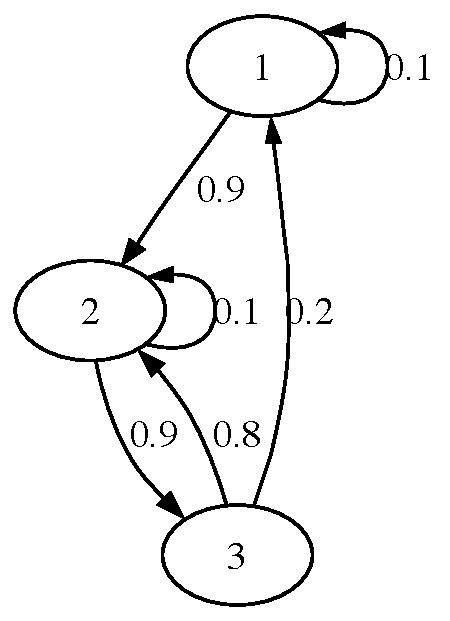
\includegraphics[scale=0.5]{smallmarkov}
  \end{minipage}
  \begin{minipage}{0.4\textwidth}
   $\displaystyle P = \left [ 
      \begin{array}{ccc} 
        0.1 & 0.9 & 0 \\ 
        0 & 0.1 & 0.9 \\ 
        0.2 & 0.8 & 0 
      \end{array} \right ]$
  \end{minipage}
  \caption{Markov process represented by a transition matrix and a graph}
  \label{fig:markovgraph}
\end{figure}

Figure~\ref{fig:markovtimeseries} shows the result of simulation of the Markov process shown in figure~\ref{fig:markovgraph} over 100 iterations.  
It is clear that the second and third states are more likely than the first.
One might reasonably enquire what the overall likelihood of a particular state would be. 

\begin{figure}[htbp]
  \centering
  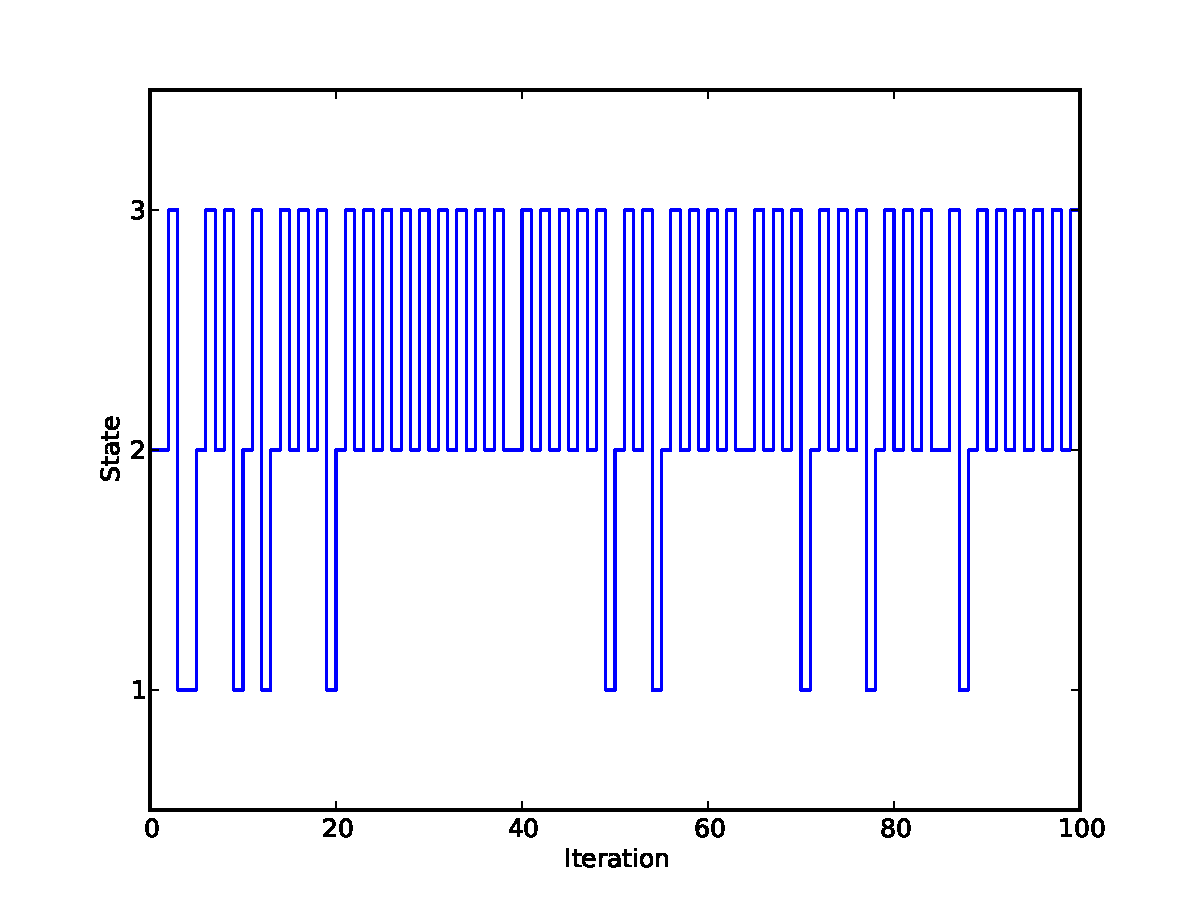
\includegraphics[width=0.8\textwidth]{simplemarkov_100_states}
  %TODO: Convert to PGF
  \caption{Time series generated by the simulation of a discrete-time Markov Model}
  \label{fig:markovtimeseries}
\end{figure}

The state transition probabilities sufficiently describe the time dependence of the process, but the initial state can not be determined using the transition probabilities alone.
The probability of the process starting out in a given state $i$ is denoted $\pi_i, i \in S$, and the vector of initial state probabilities is called
$\vect{\pi}$.
It can be seen that a discrete time Markov process is completely described by its state space $S$, its state transition matrix $P$ and its initial state probability vector $\vect{\pi}$.  
If $S$ is countable and has $N$ elements, $N^2 + N$ probabilities have to be known to fully characterise the process.
For convenience, the model is written $\lambda = (P, \vect{\pi})$.

\subsection{Transient and limiting behaviour}
Given probabilities for the current state in a row vector $\vect{p}_i$, it can be observed that the probabilities of the next state can be calculated by multiplying from the right by $P$, so that $\vect{p}_{i+1} = \vect{p}_i P$.
Repeating this procedure for a certain number of timesteps allows us to calculate the probabilities of finding the system in a particular state after those timesteps.
In this way it may be said that the $n$-step transition probability matrix $P(n) = P^n$.
Note that this means that the future probability of finding the system in a particular state can be found from a known current state by using an initial probability vector containing only one 1.

Now, if the process is allowed to evolve over time for an infinite number of timesteps, it may be asked whether the PMF approaches a limit.
If it does, this is called the limiting or steady-state distribution and we may write $\vect{p}$ = $\vect{p}P$.
Finding the limiting distribution can be posed as finding the left eigenvector of $P$ associated with a unity eigenvalue.
It is guaranteed that $P$ has a unity eigenvalue (and that this is the largest eigenvalue).
Having found this eigenvector, it is normalised such that its sum norm is 1.

\subsection{Hidden Markov Models} 
It is not always possible to observe the state (in the state space $S$) of a Markov process directly. 
It may, however, be possible to make observations from an observation space $O$ related to the state of the process.
If the probability of making a particular observation is only related to the current state of the process, the process may be described by a hidden Markov model (HMM).
What is ``hidden'' in this case are the true values of the Markov process states.

Figure~\ref{fig:hiddenmarkov} shows the situation graphically.
If the Markov process is in state 1, there are even odds that observation 2 or 3 will be made.
In state 2, only observation 2 is made and state 3 is associated with observation 1 80\% of the time and observation 2 20\% of the time.

\begin{figure}[htbp]
  \centering
  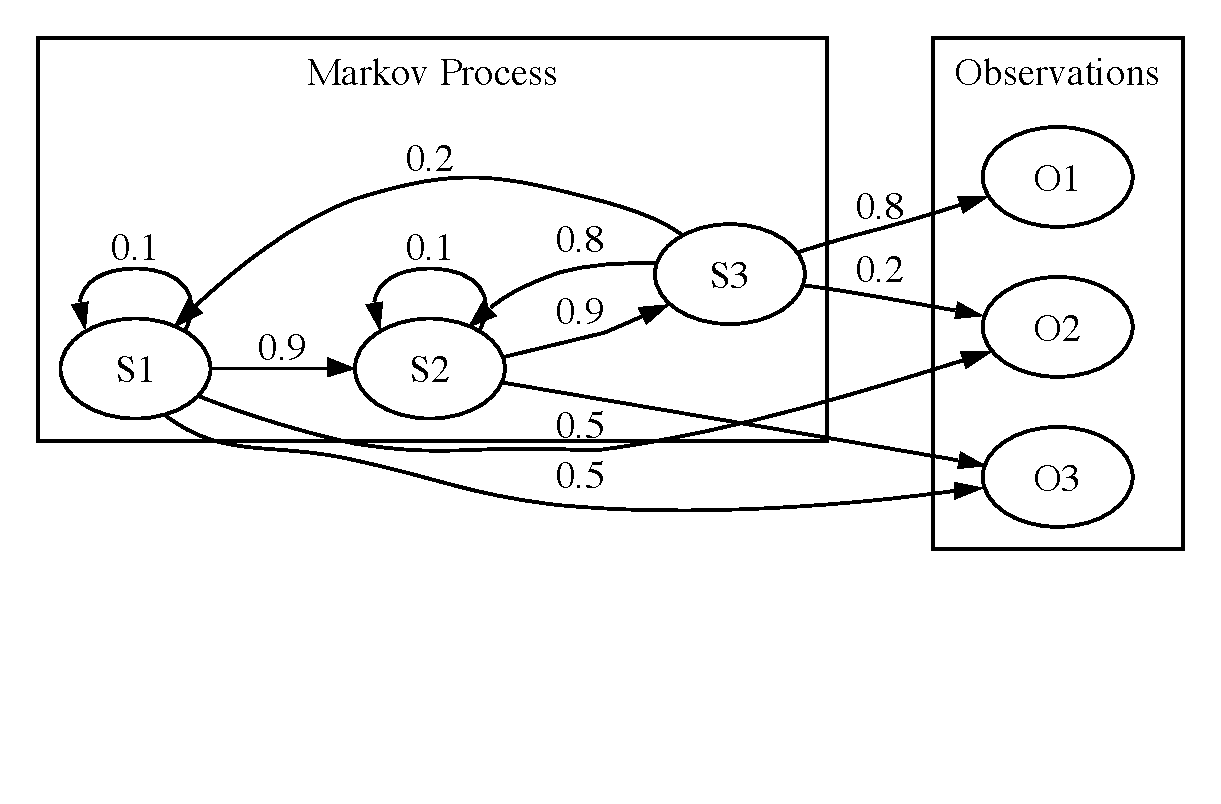
\includegraphics[scale=0.5,clip,trim=0 4cm 0 0]{smallhiddenmarkov}
  \caption{Graphical representation of a finite hidden Markov model}
  \label{fig:hiddenmarkov}
\end{figure}

The probabilities associated with a observation $k$ being made when the process is in state $i$ may be written $b_{ik}$ and can be arranged into an observation probability matrix $B$ in a similar fashion as was previously done for $P$. 
One difference is that, while $P$ was an $N \times N$ square matrix, $B$ will have $N$ rows associated with the $N$ states of the Markov process and $M$ columns associated with the observation space. 
An HMM as described here can therefore be characterised by the same $N^2+N$ probabilities describing the Markov process in addition to $MN$ observation probabilities.  
The model description can be abbreviated to $\lambda = (P, B, \vect{\pi})$.

There are three main problems associated with HMMs \citep{gamerman.lopes2006markov}:
\begin{itemize}
\item What is the probability of generating a specific output sequence from a particular model?
\item What is the most likely sequence of states that would lead to a particular output sequence? 
\item How do we identify the model that corresponds to a given output sequence?
\end{itemize}

\subsection{Continuous-time Markov Processes}
The description of discrete-time Markov processes assumed that the transition time was known or unimportant and one could imagine simulating the process by picking a state $i$ and moving to the next state with probability $p_{ij}$.  
One shortcoming of such a description is that there is no information about the amount of time a process remains in a particular state before moving to the next (or possibly same) state.  

% TODO: Flesh out this description
% look at perhaps http://www.stat.sfu.ca/~lockhart/richard/380/00_3/lectures/19/web.html
Continuous-time Markov processes encode the transition probabilities as transition rates $q_{ij}$ (forming a $Q$ matrix as $p_{ij}$ formed a $P$ matrix), such that
\begin{equation}
  \label{eq:contmarkov}
  \prob{X(t+\Delta t) = j | X(t) = i} = 
  \begin{cases}
    1 - q_{ii}\Delta t + o(\Delta t) & \text{for } i = j \\
    q_{ij}\Delta t + o(\Delta t) & \text{otherwise}
  \end{cases}
\end{equation}

The idea is that, having changed to a particular state the probability of moving to the next one approaches one over time, but at different rates.
Continuous-time Markov processes were not considered for this work due to the diffuculties in encoding the jump times for simulation.

\section{Sample Statistics}
All the properties discussed up to now have been assumed to be known values or directly calculable from known values.
In practice, however, it is common to come across data thought to be the particular values that random variables have taken on or the evolution of a stochastic process.
In such cases, it is desirable to estimate the properties discussed based on a (hopefully representative) sample.
The sampled values available will be written $\theta_i$.

The problems that present themselves are therefore
\begin{itemize}
\item Estimation of each of the statistics discussed in sections~\ref{sec:univ-rand-vari} and \ref{sec:stochastic-processes}.
\item Determination of the validity of these estimates
\end{itemize}

\subsection{Estimation}
\subsubsection{Bias}
% http://en.wikipedia.org/wiki/Bias_of_an_estimator
When a small sample is taken from a distribution, the properties of this sample are likely to deviate from the from the properties of the distribution.
Different methods of calculation can attempt to make the estimates better with regards to some criterion.
Systematic deviations from the true values are described as bias and estimates that have been developed to counter a particular deviation are called unbiased estimators.

\subsubsection{Mean}
The mean $\bar{\theta}$ of a distribution may be estimated from samples $\theta_i$ by computing the arithmetic mean
\begin{equation}
  \label{eq:mean}
  \bar{\theta} = \frac{\displaystyle \sum_{i=0}^N \theta_i}{N}
\end{equation}
This is an unbiased estimator of the mean.

\subsubsection{Variance or standard deviation}
The standard deviation of the sample (written $s_N$ for a sample size of $N$) can be naively calculated by analogy to the defintion of the variance in equation  as
\begin{equation}
  \label{eq:standardeviationsample}
  s_N = \sqrt{\frac{1}{N}\sum_{i=1}^N(\theta_i-\bar{\theta})^2}
\end{equation}
This is the maximum-likelihood estimate of the standard deviation if the sample is of a normally distributed value.
However, it underestimates the standard deviation for smaller sample sizes.
Therefore, the following unbiased estimator (called the sample standard deviation) is most commonly used:
\begin{equation}
  \label{eq:samplestandardeviation}
  s = \sqrt{\frac{1}{N-1}\sum_{i=1}^N(\theta_i-\bar{\theta})^2}
\end{equation}

\subsubsection{Skewness}
The skewness estimator is given by \citet{mooney1997monte} as:
\begin{equation} 
  \sqrt{\beta_1} =
  \frac{\displaystyle\sum_{i=1}^t \left ( \theta_i - \bar{\theta} \right
    )^3/t} { \left [ \displaystyle\sum_{i=1}^t \left (
        \theta_i-\bar{\theta} \right )^2/t \right ]^\frac{3}{2}} 
\end{equation}
\nomenclature[ga]{$\beta_1$}{Skew estimator} 
\nomenclature[ga]{$\theta$}{Vector of samples for statistical tests}

\subsubsection{Kurtosis}
The skewness estimator is usually combined with a kurtosis estimator 
\begin{equation} 
  \beta_2 =
  \frac{\displaystyle\sum_{i=1}^t \left ( \theta_i - \bar{\theta} \right
    )^4/t} { \left [ \displaystyle\sum_{i=1}^t \left(
        \theta_i-\bar{\theta} \right)^3/t \right]^2} 
\end{equation}
\nomenclature[ga]{$\beta_2$}{Kurtosis estimator}
%
In both these equations, $\bar{\theta}$ is the arithmetic mean of the samples (ie, the sum of the elements divided by $t$).  
Values of 0 and 3 for the skewness and kurtosis respectively are expected for a normal distribution~\citep{kleijnen1975statistical}.

\subsubsection{State transition probabilities}
The most direct method of estimating the state transition probabilities of a Markov process is to count the number of transitions in an input signal.
This strategy has some problems:
\begin{enumerate}
\item Certain transitions may not occur in the input signal, so that these transitions will never be simulated by the identified model
\item Segmentation of the input signal may bias the event types or transitions -- if a certain event is more often fit by the segmentation algorithm, that event will be over-represented in the transition matrix.
\end{enumerate}

If transitions between some events are very rare, it may be advisable to introduce a small artificial probability into the matrix to ensure that the event has a chance of  getting generated during the simulation.
This is especially true if the repercussions of a certain event combination are significant.  

Segmentation bias can be combated by generating a large unbiased test set and testing the segmentation algorithm on it.
If a segmentation bias is detected, the transition probabilities can be modified to take these into account.

\subsection{Verification}
It is often desired to test whether a particular sample has properties that one would expect of one were to sample a random variable with a particular CDF or PDF.
The most common tests are for normality, in other words whether the sample seems to have been drawn from a normal distribution.

\subsubsection{Shapiro-Wilk test for normality}\label{sec:shapiro-wilk-test}
The Shapiro-Wilk test~\citep{shapiro.wilk1965analysis}, calculates a W statistic that tests whether a random sample, $\theta_1, \theta_2, \dots, \theta_n$ comes from (specifically) a normal distribution.  
Small values of W are evidence of departure from normality.  
This test has done very well in comparison studies with other goodness of fit tests.

The W statistic is calculated as follows: 
\begin{equation} 
  \label{eq:shipirowilk} 
  W = \frac{
    \left( \displaystyle \sum_{i=1}^n {a_i \times \theta_i} \right)^2}
  {\displaystyle \sum_{i=1}^n 
    \left ( \theta_i - \bar{\theta} \right )^2}
\end{equation}
where the $\theta_i$ are the ordered sample values ($\theta_1$ is the smallest) and the $a_i$ are constants generated from the means, variances and covariances of the order statistics of a sample of size $n$ from a normal distribution.

\subsubsection{Kolmogorov-Smirnov test}\label{sec:kolm-smirn-test}
Further checking of normality can be done by using the Kolmogorov-Smirnov test~\citep[392--394]{chakravarti.laha.ea1967handbook} to compare the distribution to a normal distribution with the same mean and standard deviation.
This is not a specific test of normality, but rather a general goodness-of-fit test for any probability distribution.

The cumulative probability distribution curves for both distributions are plotted, and the maximum distance between them determined.  
This distance (the Kolmogorov-Smirnov distance or the KS statistic) is then compared to tables for the number of samples in the test distribution to determine the goodness of fit.  
The critical distance is also affected by the level of confidence, $\alpha$.  
It is customary to set $\alpha=\num{0.05}$, corresponding to a 5\% chance of mistakenly discarding the assumption that the test distribution is indeed normally distributed.
\nomenclature[ga]{$\alpha$}{Level of confidence in normality tests}

For samples larger than 20, the critical distance is found by calculating an asymptotic solution to an $n$\textsuperscript{th} order polynomial.  
This task is usually handled by computer software.

The Kolmogorov-Smirnov test was favoured for confirming normality of the test results as it lends itself well to graphical interpretation, enabling the tester to interpret the normality results more meaningfully than a simple number.

\section{Signal statistics}

\subsection{Ergodicity}
A process is said to be ergodic if the properties of the distributions the points are drawn from do not change over time.  
More specifically, a process may be said to be mean ergodic or ergodic to the mean if $E(X)=\mu$ is the same for all times.

It is possible to estimate the mean of an ergodic process by 
\begin{equation}
  \hat{\mu_T} = \frac{1}{2T} \int_{-T}^{T} x(t) \dd t
\end{equation}


% Local Variables:
% TeX-master: "thesis"
% End:

